

\documentclass[letterpaper,twocolumn,amsmath,amssymb,prb]{revtex4-1}
\usepackage{graphicx}% Include figure files
\usepackage{dcolumn}% Align table columns on decimal point
\usepackage{bm}% bold math
\usepackage{color}

%%%%%%%%%%%%%%%%%%%%%%%%%%%%%%%%%%%%%%%%%%%%%%%%%%%%%%%%%%%%
%% Definitions
\def\re{\text{Re}}
\def\im{\text{Im}}
\def\ket#1{\vert #1 \rangle}
\def\cU{{\cal{U}}}
\def\cD{{\cal{D}}}
\def\re{\text{Re}}
\def\im{\text{Im}}
\newcommand{\red}[1]{{\bf \color{red} #1}}
\newcommand{\blue}[1]{{\bf \color{blue} #1}}
\newcommand{\green}[1]{{\bf \color{green} #1}}
\newcommand{\rr}{\textbf{r}}
\newcommand{\xx}{\textbf{x}}
\newcommand{\refnote}{\red{[ref]}}

\newcommand{\fixme}[1]{\red{[#1]}}

% needsworklater is used to annotate bits that need work, but that we
% can postpone for a while.
\newcommand{\needsworklater}[1]{\emph{[#1]}}
% needsworknow is intended to prioritize stuff that needs fixing.
\newcommand{\needsworknow}[1]{\textcolor{red}{[\emph{#1}]}}

%%%%%%%%%%%%%%%%%%%%%%%%%%%%%%%%%%%%%%%%%%%%%%%%%%%%%%%%%%%%

\begin{document}
\title{A Classical Density-Functional Theory for Describing Water Interfaces}

\author{Jessica Hughes}
\affiliation{Department of Physics, Oregon State University, Corvallis, OR
97331}

\author{David Roundy}
\affiliation{Department of Physics, Oregon State University, Corvallis, OR
97331}

%%%%%%%%%%%%%%%%%%%%%%%%%%%%%%%%%%%%%%%%%%%%%%%%%%%%%%%%%%%%
\begin{abstract}
\needsworklater{ We develop a classical density functional theory for
  water by combining the fundamental-measure theory functional--which
  describes hard sphere fluids--with attractive interactions based on the 
  Statistical Associating Fluid Theory (SAFT).  Using
  this approximation, we are able to describe various properties of
  water near liquid-vapor and liquid-solid interfaces, including water confined 
  to a hard-walled slit and hydrophobic rods immersed in water.  This functional 
  will be the foundation for a efficient method for future work
  predicting the interactions of chemicals in aqueous solution on an
  atomic level.}

\tableofcontents
\end{abstract}

\maketitle

%%%%%%%%%%%%%%%%%%%%%%%%%%%%%%%%%%%%%%%%%%%%%%%%%%%%%%%%%%%%
\section{Introduction}

\subsection{Water---the universal solvent}

The simple yet complex water molecule is one of the most important 
substances for life and industry. The structure and geometry of the 
water molecule leads to a strong polarity and complex intermolecular
forces. The hydrogen bonds formed by water are very strong, creating
tetragonal clusters (CITE?) that lead to many of water's unusual properties,
such as the high melting, boiling, and critical temperatures.
The large dielectric constant (D$\sim$80) (CITE) is partially responsible for
water as a universal solvent, along with the ease of availability and use.

\subsection{Classical density-functional theory}

It is challenging to describe all the relevant properties of water using
a model, especially if a low computational cost is also desired.

Some models, including SAFT, are designed for use with
homogeneous systems only. Although these models are useful, much of the interesting
chemistry that occurs in water cannot be described with a homogeneous only model. To
describe solvation and other processes in aqueous solution, a more robust theory is 
needed.

Classical density-functional theory (DFT) provides an efficient way to evaluate the
free energy using the density of the fluid. The free energy is a functional of the 
density function and is independent of any external potentials\cite{ebner1976}. 
Mermin\cite{mermin1965thermal} gives a theorem extending that of Hohenberg and 
Kohn\cite{hohenberg1964inhomogeneous} to nonzero temperatures:
\begin{equation}
  A(T) = \underset{n(r)}{min}\left\{ F[n(r),T] + \int V_{ext}(r) n(r) d^3r\right\}
\end{equation}
This is the basis for classical DFT, which can be used with a variety of external potentials, 
from the simple interaction with a 
hydrophobic wall to the complex strong interaction with hydrophilic solutes.

%%%%%%%%%%%%%%%%%%%%%%%%%%%%%%%%%%%%%%%%%%%%%%%%%%%%%%%%%%%%
\section{Theory and Methods}
We introduce a new classical density functional for water that
predicts the \needsworklater{vapor density, liquid density, bulk
  modulus, and bulk surface tension, as well as allows for
  liquid-vapor coexistence}.  The Helmholtz free energy functional is
based on SAFT, and is composed of the usual terms:
\begin{equation}
  F[n] = F_\textit{id}[n] + F_\textit{hs}[n]  +
F_\textit{disp}[n]+ F_\textit{assoc}[n],
\end{equation}
where $F_\textit{id}$ is the ideal gas free energy, $F_\textit{hs}$ is
a hard-sphere free energy, $F_\textit{assoc}$ is the free energy of
association, and $F_\textit{disp}$ is the dispersion energy.  In
addition, a chemical potential term is used, so we actually work in
the grand canonical ensemble.  In the following sections, we will
introduce the terms of this functional.

\subsection{Ideal gas functional}
The first term is the ideal gas free energy functional,
which incorporates effects of kinetic energy.  The ideal gas
functional is given by
\begin{equation}\label{idealgas}
  F_{id}[n] = k_B T \int n(\xx)\left( \ln{n(\xx)} - 1\right) d\xx
\end{equation}
where n(\xx) is the density of water molecules.  The ideal gas free
energy functional has the property that the contact density at a hard
surface $n_c$ is proportional to the pressure on that surface,
according to the contact value theorem
\begin{equation}\label{contactvaluethm}
  p = n_c k_BT \:,
\end{equation}
which also leads to the property that the free energy of solvation of
a hard solute is proportional to its volume in the limit of small
solutes.  These properties are retained by the total functional,
provided the remaining terms are \emph{purely
  nonlocal}~\cite{ashcroft?}.

\subsection{Hard-sphere repulsion}

We model the repulsive interactions using the White Bear version of
the Fundamental-Measure Theory~(FMT) functional for the hard-sphere
fluid~\cite{roth2002whitebear}.  In the homogeneous limit, the White
Bear functional reduces to the Mansoori-Carnahan-Starling-Leland
equation of state.  FMT functionals are expressed as the integral of
the \emph{fundamental measures} of a fluid, which provide local
measures of quantities such as the packing fraction, density of
spheres touching a given point and mean curvature.  The excess free
energy is written as:
\begin{equation}
F_{hs}[n] = k_B T \int (\Phi_1(\xx) + \Phi_2(\xx) + \Phi_3(\xx)) d\xx \; ,
\end{equation}
with integrands
\begin{align}
\Phi_1 &= -n_0 \ln\left( 1 - n_3\right)\\
\Phi_2 &= \frac{n_1 n_2 - \mathbf{n}_{V1} \cdot\mathbf{n}_{V2}}{1-n_3} \\
\Phi_3 &= (n_2^3 - 3n_2 \mathbf{n}_{V2} \cdot \mathbf{n}_{V2})
  \frac{
    n_3 + (1-n_3)^2\ln(1-n_3)
  }{
    36\pi n_3^2\left( 1 - n_3 \right)^2
  } ,
\end{align}
where the fundamental measure densities are given by:
\begin{align}
  n_3(\xx) &= \int n(\xx') \Theta(\left|\xx - \xx'\right| - R) d\xx' \\
  n_2(\xx) &= \int n(\xx') \delta(\left|\xx - \xx'\right| - R) d\xx'
  \\
  \mathbf{n}_{V2} &= \mathbf{\nabla} n_3 \\
  n_1 &= \frac{n_2}{4\pi R}\\
  \mathbf{n}_{V1} &= \frac{\mathbf{n}_{V2}}{4\pi R}\\
  n_0 &= \frac{n_2}{4\pi R^2}
\end{align}
For our water functional, we use the hard-sphere radius of
3.03420~\AA, which was found to be optimal by Clark
\emph{et al}.\cite{clark2006developing}

\begin{figure}
\begin{center}
\includegraphics[width=\columnwidth]{figs/equation-of-state}
\end{center}
\caption{The theoretical versus experimental phase diagram, vapor
  pressure versus temperature.  }
\label{fig:equation-of-state}
\end{figure}

\subsection{Association free energy}
The first attractive energy term is the association term, which
accounts for hydrogen bonding.  Hydrogen bonds are modeled as four
attractive patches (``association sites'') on the surface of the hard
sphere.  These four sites represent two protons and two electron lone
pairs.  There is an attractive energy $\epsilon_\textit{assoc}$ when
two molecules are arranged such that the proton of one overlaps
with the lone pair of the other.  The volume over which this
interaction occurs is $\kappa_\textit{assoc}$, giving the association
term in the free energy has two empirical parameters that are fit to
experimental data.

The association functional we use is a modified version of that of Yu
and Wu\cite{yu2002fmt-dft-inhomogeneous-associating}.\footnote{We
  should note that Fu and Wu\cite{fu2005vapor-liquid-dft} use almost
  the same functional, but their paper contains errors in the
  association term and is not useful as a reference.}  The functional
of Fu and We includes the effects of density inhomogeneities on the
\emph{contact density} of hard spheres, which conventionally appears
in the form of the density multiplied by the contact value of the
correlation function $g^{HS}_\sigma$, but is based on the SAFT-HS
equation of state\cite{FIXME}, rather than the SAFT-VR equation of
state\cite{gil-villegas-1997-SAFT-VR} which is used in the optimal
SAFT parametrization for water found by Clark \emph{et
  al}\cite{clark2006developing}.

The association free energy for our four-site model has the form
\begin{align}
  F_\text{assoc}[n] &= 4 k_BT \int n_0(\xx)
  \left(\ln X(\xx) - \frac{X(\xx)}{2} + \frac12\right) d\xx
\end{align}
where the value of $4$ comes from the four association sites per
molecule, and the functional $X$ is the fraction of assotiation sites
\emph{not} hydrogen-bonded.  The fraction $X$ is determined by the
quadratic equation
\begin{align}
  X(\xx) &= \frac{\sqrt{1 + 8n_0(\xx)\zeta(\xx)\Delta(\xx)} - 1}
  {4 n_0(\xx)\zeta(\xx)\Delta(\xx)}
\end{align}
where the factor $\zeta$ from
Yu and We\cite{yu2002fmt-dft-inhomogeneous-associating,
  fu2005vapor-liquid-dft} describes the inhomogeneity of the fluid
density, and reduces to unity in the homogeneous limit.
\begin{align}
  \zeta(\xx) &= 1 - \frac{\mathbf{n_{2V}}\cdot\mathbf{n_{2V}}}{n_2^2}
\end{align}
The functional $\Delta$ is a measure of the hydrogen-bonding
probability.  In the SAFT-VR model\cite{gil-villegas-1997-SAFT-VR}, $\Delta$ is
given by
\begin{align}
  \Delta &= \kappa_\textit{assoc} g^\textit{SW}_\sigma
  \left(e^{-\beta\epsilon_\textit{assoc}} - 1\right) \\
  g^\textit{SW}_\sigma &= g^\textit{HS}_\sigma +
  \frac{1}{4}\beta\left(\frac{\partial a_1}{\partial n_3} -
  \frac{\lambda}{3 n3}\frac{\partial a_1}{\partial \lambda}\right)
\end{align}
% This is equation 77 of gil-villegas-1997-SAFT-VR
where $g^\textit{SW}_\sigma$ is the correlation function evaluated at
contact for a hard-sphere fluid with a square-well attractive
potential, and $a_1$ and $a_2$ are two terms in the dispersive term of
the free energy.  The correlation function $g^\textit{SW}_\sigma$ is
written as a perturbative correction to the hard-sphere correlation
function, for which we use the functional of Yu and
Wu.\cite{yu2002fmt-dft-inhomogeneous-associating}
\begin{align}
  g_\sigma^{HS} &= \frac{1}{1-n_3}
  +\frac32\frac{\zeta}{(1-n_3)^2}
  + \frac12\frac{n_3^2\zeta}{(1-n_3)^3}
\end{align}

% \begin{figure}
% \begin{center}
% \includegraphics[width=\columnwidth]{figs/saturated-liquid-density}
% \end{center}
% \caption{The theoretical versus experimental saturated liquid density
%   versus temperature.  }
% \label{fig:saturated-liquid-density}
% \end{figure}

\subsection{Dispersion free energy}
The final term in the free energy is the dispersion term.  We use a
dispersion term based on the SAFT-VR
approach\cite{gil-villegas-1997-SAFT-VR}, which has two free
parameters, an interaction energy $\epsilon_\textit{disp}$ and a
length scale $\lambda_\textit{disp}$.

The dispersion free energy has the form~\cite{gil-villegas-1997-SAFT-VR}
\begin{align}
  F_\text{disp} &= A_1 + \beta A_2
\end{align}
where $A_1$ and $A_2$ are the first two terms in a high-temperature
perturbation expansion.  $A_1$ is the mean-field dispersion
interaction, which for a homogeneous fluid is given by
\begin{align}
  A_1 &= \frac12 n_b \int \varphi(\left|\xx\right|)
  g_{HS}(\left|\xx\right|) d\xx
\end{align}
The second dispersion term in the free energy $A_2$ describes the
effect of fluctuations resulting from the compression of the fluid due
to the dispersion interaction itself, and is commonly approximated
using the local compressibility approximation (LCA).

We use a free square-well function for the dispersion $\varphi$, which
has been demonstrated \textcolor{red}{(CITE)} to give a reasonable fit
to the equation of state.  Thus our model interaction has the form:
\begin{equation}
  \varphi(r) = \Theta(r-2 \lambda_\textit{disp} R)
\end{equation}
where $\Theta$ is the Heaviside step function.

\textcolor{red}{TODO:  Add the actual functions that we use and the
  actual form.  The above is really just an introduction.}


\begin{figure}
\begin{center}
\includegraphics[width=\columnwidth]{figs/temperature-versus-density}
\end{center}
\caption{The theoretical versus experimental temperature versus density. }
\label{fig:temperature-vs-density}
\end{figure}

% \begin{figure}
% \begin{center}
% \includegraphics[width=\columnwidth]{figs/entropy}
% \end{center}
% \caption{The free energy, internal energy, and temperature*entropy 
% versus density at room temperature.  }
% \label{fig:energy-room-temp}
% \end{figure}

\subsection{Other thermodynamic functions}

From the Helmholtz free energy functional, we may obtain any other
thermodynamic functions we should choose.  The grand free energy
$\Phi$, which we ordinarily use in our computations, is obtained by
simply adding a chemical potential term:
\begin{equation}
  \Phi[n] = F[n] + \mu \int n(\xx) d\xx
\end{equation}

The pressure would naturally be obtained by taking a partial
derivative with respect to volume at fixed temperature.  Since
\emph{volume} isn't a parameter in density-functional theory, we
consider the \emph{free energy per unit volume}.
\begin{align}
  F[n] &= f[n]V \\
  p[n] &= -\left(\frac{\partial F[n]}{\partial V}\right)_{T} \\
  &= -\left(\frac{\partial f[n]V}{\partial V}\right)_{T} \\
  &= -V\left(\frac{\partial f[n]}{\partial V}\right)_{T}
   - f[n]\left(\frac{\partial V}{\partial V}\right)_{T} \\
  &= n \left(\frac{\partial f[n]}{\partial n}\right)_{T} - f[n]
\end{align}

\begin{figure}
\begin{center}
\includegraphics[width=\columnwidth]{figs/pressure-with-isotherms}
\end{center}
\caption{The pressure versus density for various temperatures, including
experimental pressure data from NIST\cite{nistwater}. The dash-dotted lines
indicate the computationally calculated pressure and the open circles are 
NIST data points, plotted for every other isotherm. The solid and dotted lines
represent the theoretical and experimental coexistence curves.}
\label{fig:pressure-with-isotherms}
\end{figure}

Figure \ref{fig:pressure-with-isotherms} shows the calculated pressures for
isotherms ranging from room temperature to past the critical temperature. The solid 
line is the theoretical coexistence curve calculated from the SAFT functional. 
For a given isotherm, the pressure curve should intersect this coexistence curve 
twice, at the values of the vapor and liquid densities. The functional matches well with
the experimental data from NIST away from the critical point. The slope of the pressure
versus density curve is proportional to the compressibility, which is close but slightly too
large at room temperature. 

The entropy is naturally obtained by taking a partial derivative with
respect to temperature:
\begin{align}
  S[n] &= \left(\frac{\partial F[n]}{\partial T}\right)_{V}
\end{align}
This derivative is trivial for the ideal gas and hard sphere free
energies, which are simply proportional to the temperature.  For the
association and dispersion free energies, it is a little more work,
but still not hard.

Once we have the entropy, finding the internal energy is a simple
matter of subtraction:
\begin{align}
  U[n] &= F[n] + TS[n]
\end{align}
and the enthalpy is not much more work:
\begin{align}
  H[n] &= F[n] + TS[n] + pV
\end{align}

The calculated heat of vaporization at atmospheric pressure is
$\Delta H_{vap}$= 39.41 kJ/mol at the normal boiling point of water,
373 K. This compares well to the experimental
value measured by NIST ($\Delta H_{vap}$= 40.65 kJ/mol\cite{nistwater}), with 
an error of only a few percent.

\begin{figure}
\begin{center}
\includegraphics[width=\columnwidth]{figs/finding-vapor-pressure}\\
\includegraphics[width=\columnwidth]{figs/near-critical-point}
\end{center}
\caption{By plotting the free energy vs. density it is possible to
  determine a saturated liquid or vapor state by the common tangent
  method.  }
\label{fig:homogeneous}
\end{figure}

\begin{figure}
\begin{center}
\includegraphics[width=\columnwidth]{figs/surface-tension}
\end{center}
\caption{The theoretical versus experimental surface tension
  versus temperature. The experimental data is taken from NIST.\cite{nistwater} }
\label{fig:surface-tension}
\end{figure}

\begin{figure}
\begin{center}
\includegraphics[width=\columnwidth]{figs/surface-298}
\end{center}
\caption{Liquid-vapor interface profile at room temperature.  }
\label{fig:liquid-vapor-profile}
\end{figure}

\subsection{Determining the empirical parameters}\label{sec:empirical}

The majority of the empirical parameters used in our functional are
taken from the paper of Clark \emph{et al} on developing an optimal
SAFT model for water\cite{clark2006developing}.  This SAFT model
contains five empirical parameters: the hard-sphere radius, an energy
and length scale for the dispersion interaction, and an energy and
length scale for the association interaction.  In addition to the five
empirical parameters of Clark \emph{et al}, we add a single additional
parameter defining the length scale over which the density is averaged
when computing the dispersion free energy.  We use this final
parameter to fit the surface tension, with the result shown in
Figure~\ref{fig:surface-tension}.  Because the SAFT model of Clark
\emph{et al} overestimates the critical temperature---which is a
common feature of models which do not explicitly treat the critical
point---we cannot correctly describe the surface tension at all
temperatures, and chose to fit it for the temperature range at which
water is liquid at one atmosphere of pressure.

\fixme{I'm not sure if this paragraph belongs here.  Somewhere I think
  it's worth discussing any of these homogeneous plots we include, and
  this might be the right place.  We also might want to include one or
  more of them earlier in the text.  A general rule is that any figure
  that is included should be referenced in the text.  If there's
  nowhere in the text that it fits, then it probably doesn't belong in
  the paper....  So I'm not removing the follwoing bits since it's up
  to you, Jess, whether to remove the figures.  We should
  \emph{definitely} remove some of them.}  For reference, we plot the
predicted vapor pressure (see Figure~\ref{fig:equation-of-state}) and
coexistence curve (see
Figure~\ref{fig:temperature-vs-density}) against experimental
values.  To find the densities, we use the ``common tangent'' rule,
as illustrated in Figure~\ref{fig:homogeneous}.

% \begin{table}
% \begin{tabular}{ccc}
%   Fitting Parameters& \hspace{2em} & Experimental Values\\
% \begin{tabular}{cc}
%   $R$ & 2.3 $a_o$ \\
%   $A$ & -0.0100909 Hartree \\
%   $\gamma$ & 5\\
%   $V$ & 515.792 $a_o^3$  \\
%   $b$ & 0.75 $a_o$ \\
%   $\mu$ & -0.014063 Hartree 
% \end{tabular}
% && 
% \begin{tabular}{cc}
%  $n_l$ & 4.939 $\times 10^{-3} a_o^{-3}$\\
%  $n_v$ & 1.141 $\times 10^{-7} a_o^{-3}$\\
%  $\sigma$ & ??? \\
%  $B$ & $7.435\times 10^{-5}$ Hartree$/a_o^3$\\
%  $T$ & 298.15 K \\
% \end{tabular}
% \end{tabular}
% 
% \caption{Empirical parameters of optimized functional and experimental
%   values matched, where $a_o$ is the Bohr radius, and $\sigma$ is the
%   surface tension.  This table is not yet complete, but it should
%   be soon...  We'll also need to think about the best units to use
%   here.  Atom units might be best, but it also might be better to
%   consistently use eV and angstrom or something.  I'm not sure about
%   putting $k_BT$ data in the table.  Maybe it belongs in the caption?}
% \label{tab:parameters}
% \end{table}

%%%%%%%%%%%%%%%%%%%%%%%%%%%%%%%%%%%%%%%%%%%%%%%%%%%%%%%%%%%%
\section{Results and discussion}

\subsection{Water confined to a slit}

\begin{figure}
\begin{center}
\includegraphics[width=\columnwidth]{figs/density-1D}
\includegraphics[width=\columnwidth]{figs/energy-1D}
\end{center}
\caption{ Density profile (top) and 
energy densities (bottom) for a slab of water with molecules 
constrained to move in one dimension. The free energy, internal energy
and entropic energy densities are shown for a slit size of 4.0 nm. The dashed
line in the top figure represents the saturated liquid density.}
\label{fig:energy-1D}
\end{figure}

The fluid density at a liquid-solid interface commonly displays
oscillatory behavior, but the presence of density oscillations at
liquid-vapor interfaces is more debated\cite{penfold2001structure}.
In fact, the \emph{meaning} of the density profile at a liquid-vapor
interface is clouded by the existence of long-wavelength perturbations
known as \emph{capillary waves}.  These waves are not accounted for in
density-functional theory (although the \emph{exact}
density-functional theory \emph{would} include them), with the result
that the density profile will be smoothed out by CW effects. The liquid-vapor
interface is plotted in Figure \ref{fig:liquid-vapor-profile} and shows
some small oscillations.

One of the most computationally simple ways to study confined water is by
constraining it to a slit where the water molecules can only move in one
dimension. Experimentally, this could represent two different situations.
The first, water between two perfectly aligned and smooth planes, is not common 
in experiment due to the difficulty of creating such an ideal situation. The
second
possibility is a large sphere brought close to a plane, which eliminates the 
need for perfect alignment.

We choose a chemical potential corresponding to a pressure of 1 atm and set the
temperature to a typical room temperature of 298 K. We apply 
a constraining potential outside the slit, where we choose a small non-zero
density for numerical reasons. The slits studied range in size from 0.1 nm to 
8.0 nm. We minimize the energy and calculate density, energy, and $X$ on a
lattice
with a spacing of approximately 0.01 nm (0.2 bohrs) between lattice points.

The density profile for a slit of size 4.0 nm is shown in Figure
\ref{fig:energy-1D}. Near the interface, there are oscillations around the
liquid density which decrease near the center of the slit. We expect the center
of the slit to act approximately like bulk water, and the absence of
oscillations supports this. For larger slits (6.0 nm or more) the majority of
the water molecules in the slit act like the bulk. Based on our computations, we
also determine the smallest slit that can contain liquid water. This result is
approximately 0.6 nm. For smaller slits, the initial liquid water inside will
vaporize. The results for larger liquid-filled slits are only metastable,
however,as a vapor-filled slit is thermodynamically favorable. Based on our
calculations for a pressure of 1 atm, the work needed to pull apart
the two hard walls comprising the slit is one to two orders of magnitude less
than the free energy of the liquid-filled slit. For the range of slit sizes we
studied (0.1 to 8.0 nm), all the computational results of liquid-filled are
metastable. Lum, Chandler and Weeks \cite{lum1999hydrophobicity} discuss the
stability of water between large hydrophobic plates and the critical separation
necessary for stability. For water at room temperature and atmospheric pressure,
plates with a separation smallerthan about 100 nm will not contain stable liquid
water. They go on to say that confined water has a region of metastability down
to separations of about 5 nm. This is comparable to the slit separation where
our calculations show water inside the slit acting like the bulk liquid, which
we know to be a metastable solution. Forsman et al.\cite{forsman1996computer}
also study water between two hard walls at constant chemical potential. They 
also conclude that the liquid state is likely metastable, and there is a free
energy barrier to reach the stable vapor phase. 

\begin{figure}
\begin{center}
\includegraphics[width=\columnwidth]{figs/xassoc-1D}
\end{center}
\caption{The number of hydrogen bonds per molecule for a slab of water 
with molecules constrained to move in one dimension. Each molecule may contribute to
four bonds, although each bond involves two molecules so to calculate the actual 
number of bonds there would be another factor of 2.}
\label{fig:xassoc-1D}
\end{figure}

The value of $X$ behaves as expected for water constrained to a slit. We
show in Figure \ref{fig:xassoc-1D} the number of hydrogen bonds per water 
molecule, equal to $4(1-X)$, for a slit of 4.0 nm.
Outside the slit, there is no hydrogen bonding and inside the number of hydrogen
bonds is approximately equal to 3.5, which is expected for saturated liquid water.

\subsection{One hydrophobic rod}

We move into two dimensions by studying a single hydrophobic rod
immersed in water. Figure \ref{fig:density-single-rod} shows density
profiles for three different radii, 0.3 nm, 0.5 nm, and 1 nm. There are the
expected oscillations outside the rod and as the distance away from the rod increases
the density approaches that of the bulk saturated liquid density. The small radius
rod has comparatively larger oscillations and a higher contact density.

\begin{figure}
\begin{center}
\includegraphics[width=\columnwidth]{figs/density-single-rod}
\end{center}
\caption{ Density profiles for a single rod of different radii. The dotted line
represents the saturated liquid density.  }
\label{fig:density-single-rod}
\end{figure}

\begin{figure}
\begin{center}
\includegraphics[width=\columnwidth]{figs/energy-vs-diameter}
\end{center}
\caption{ Energy versus diameter for a single hydrophobic rod
immersed in water. This should have an asymptote equal to the surface
tension at room temperature, and it agrees well with the surface tension in Figure 
\ref{fig:surface-tension}. (FIX - 0.4 nm?) }
\label{fig:energy-vs-diameter}
\end{figure}

\subsubsection{Resolution and convergence tests}

Figure \ref{fig:densityresolution} shows the density profiles for three different
values of the lattice spacing resolution. The density oscillations around a single
rod of radius 0.5 nm look nearly identical for all resolutions except for the first peak. 
This contact density is important as it will be proportional to the pressure on the 
rod\ref{contactvaluethm}. The 
contact density calculated using the medium resolution is within less than 4\% of the value at
high resolution, while the low resolution contact density is off by about 5\%. There is some
uncertainty in the value of contact density due to the different lattice spacings. The total
free energy calculations compare much more favorably. The medium resolution is within 
0.5\% and the low resolution is within 1\% of the high resolution free energy.


\begin{figure}
\begin{center}
\includegraphics[width=\columnwidth]{figs/density-vs-radius}
\end{center}
\caption{ Density profiles for 
a single hydrophobic rod with a radius of 0.5 nm using several different 
lattice spacing resolutions. We used a high resolution of 0.05 bohrs ($\approx$ 0.003 nm), 
medium 0.2 bohrs ($\approx$ 0.001 nm), and low 0.5 bohrs ($\approx$ 0.03 nm).}
\label{fig:densityresolution}
\end{figure}

\subsection{Hydrophobic interaction of two rods}

Here we will want to cite~\cite{walther2004hydrodynamic}, which gives
simulations for two interacting nanotubes in water.  It's not
precisely the same, but if we can't find something more similar, this
would be worth citing.

% \begin{figure}
% \begin{center}
% \includegraphics[width=\columnwidth]{figs/density-rods-in-water}
% \end{center}
% \caption{ Density profile for two hydrophobic rods (diameter 1.0 nm) at a 
% separation of 0.8 nm. The scale on the right is density in g/mL.}
% \label{fig:density-rods}
% \end{figure}

\begin{figure}
\begin{center}
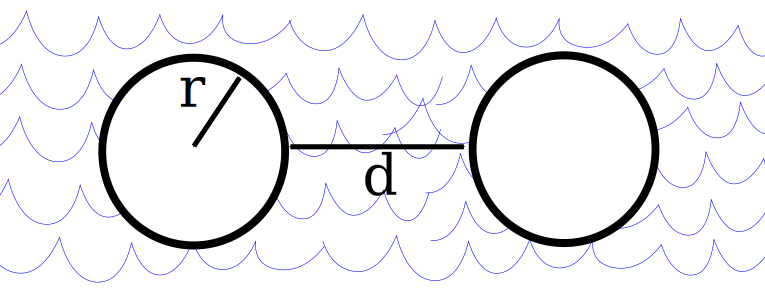
\includegraphics[width=\columnwidth]{figs/rods-diagram}
\end{center}
\caption{ Cross section schematic for two hydrophobic rods immersed in water.
The radius and separation are shown.}
\label{fig:rods}
\end{figure}

\begin{figure}
\begin{center}
\includegraphics[width=\columnwidth]{figs/rods-energy-vs-distance}
\end{center}
\caption{ Energy versus separation for two identical hydrophobic rods with diameters
of 1.0 nm. }
\label{fig:rods-energy-vs-distance}
\end{figure}


%%%%%%%%%%%%%%%%%%%%%%%%%%%%%%%%%%%%%%%%%%%%%%%%%%%%%%%%%%%%
\section{Conclusion}

[conclusion text]

\bibliography{paper}% Produces the bibliography via BibTeX.

\end{document}

